The PRISM tool can evaluate a wide range of dependability properties. In this work, we are particularly interested in evaluating signal transmission performance, specifically focusing on scenarios where the individual experiencing distress maintains a good psychological status. The source code of our artifacts is available in \cite{newcas2025}.

	    \begin{resp}{\textbf{\textit{Property}}}
        \begin{equation}
        \label{eq1}\tag{Rescue}
         \mathtt{ P=? [ (s=\quot{\textcolor{red}{Rescued} }) \  U^{\leq T} \ !(s=\quot{\textcolor{red}{Rescued} })  ]} 
        \end{equation}
        \end{resp}
        \normalsize
        
In Property \ref{eq1}, we evaluate signal performance by calculating the probability that the satellite successfully collects the signal from a beacon, transmits it through FLS services, initiates an RLM request, alerts a rescue coordination center, and ultimately ensures the correct provision of RLS services. The label \quot{\textcolor{red}{\emathtt{Rescued}}} refers to the state where the satellite collects the signal sent by the person in distress. This successful rescue scenario requires the conjunction of several conditions to be met: 
\begin{enumerate}
\item The detection performance must be in the nominal state (\emathtt{SAR\_DETECTION\_S \geq Nominal}).
\item The FLS status must be nominal (\emathtt{SAR\_FLS\_S \geq Nominal}).
\item The RLS service must also be in a nominal state (\emathtt{SAR\_RLS\_S \geq Nominal}).
\end{enumerate}

\noindent
    \begin{figure}[!htb]
    \centering
       \begin{tabularx}{\linewidth}{ m{8cm} }
           
\noindent
 \begin{minipage}[t]{8cm}
     \centering

    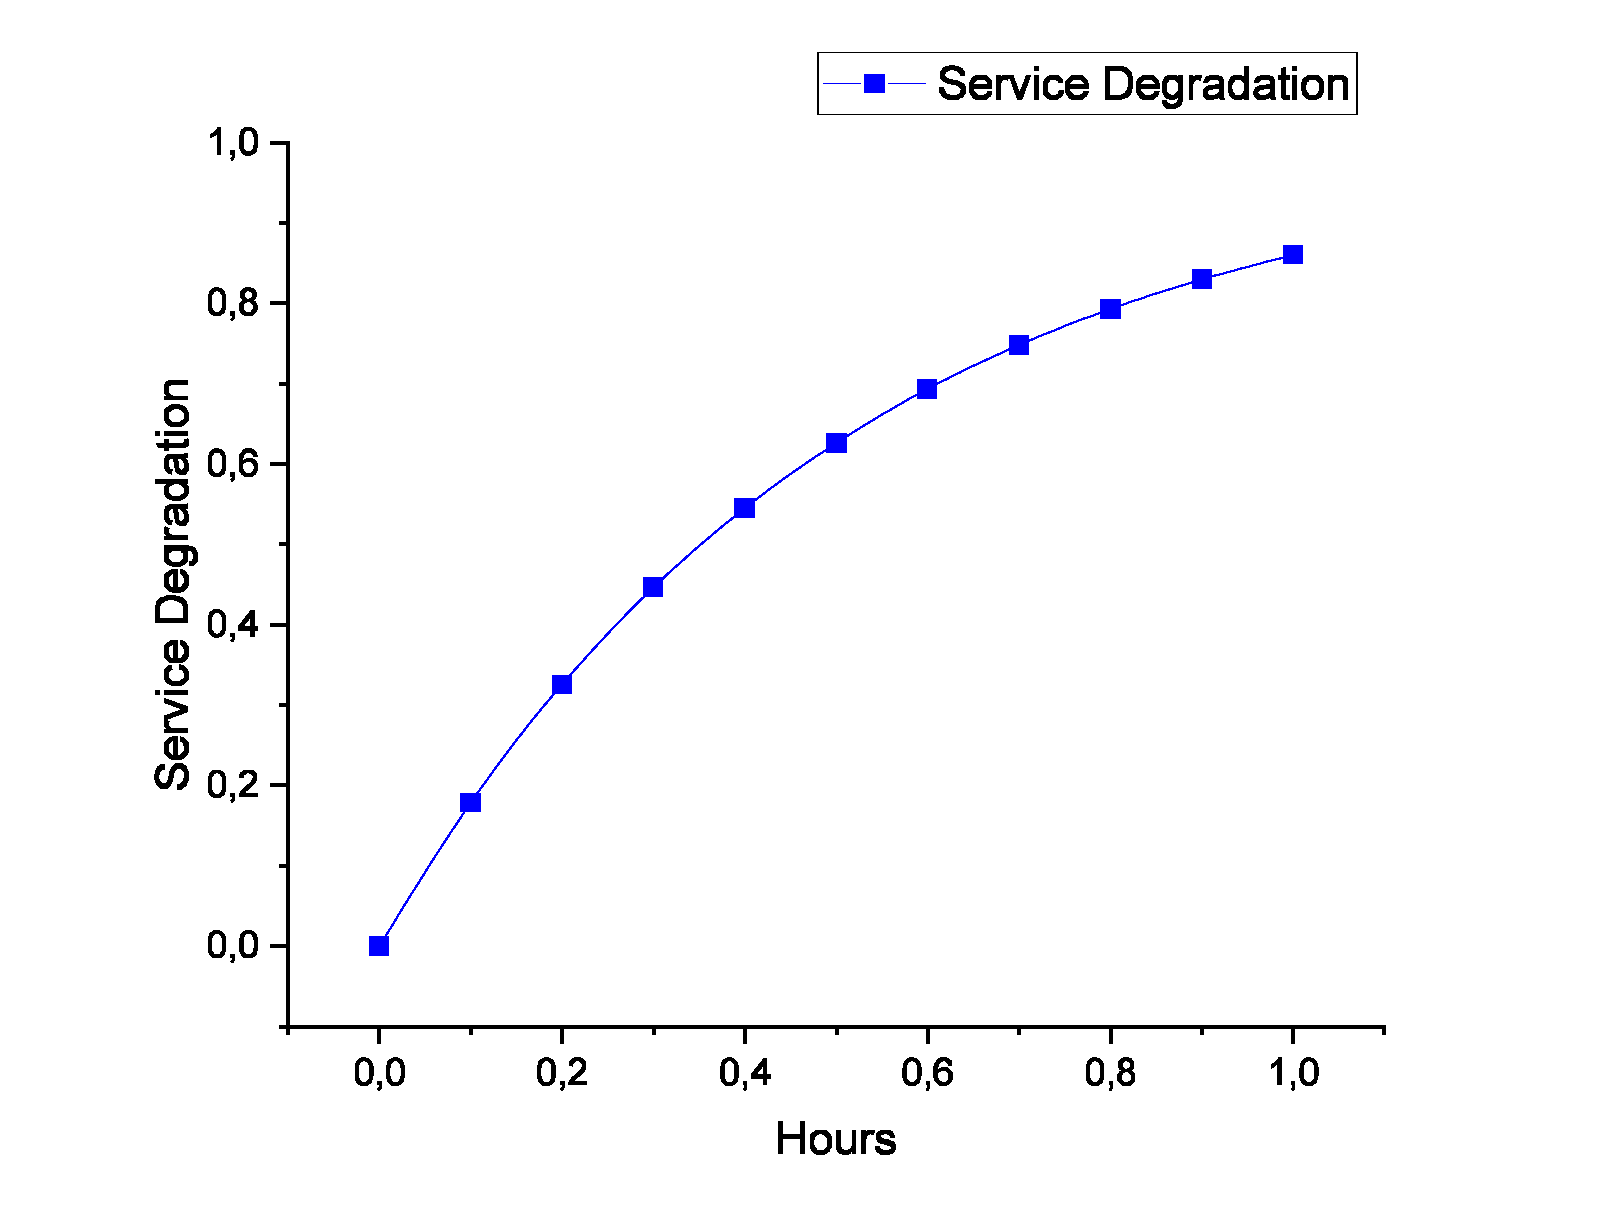
\includegraphics[width=250pt, height =180pt]{Graph2.pdf}
    \caption{Verification of Property \ref{eq1}.}
    \label{fig:01}
   \end{minipage}
    
          \\
\noindent
   \begin{minipage}[t]{8cm}
     \centering
   		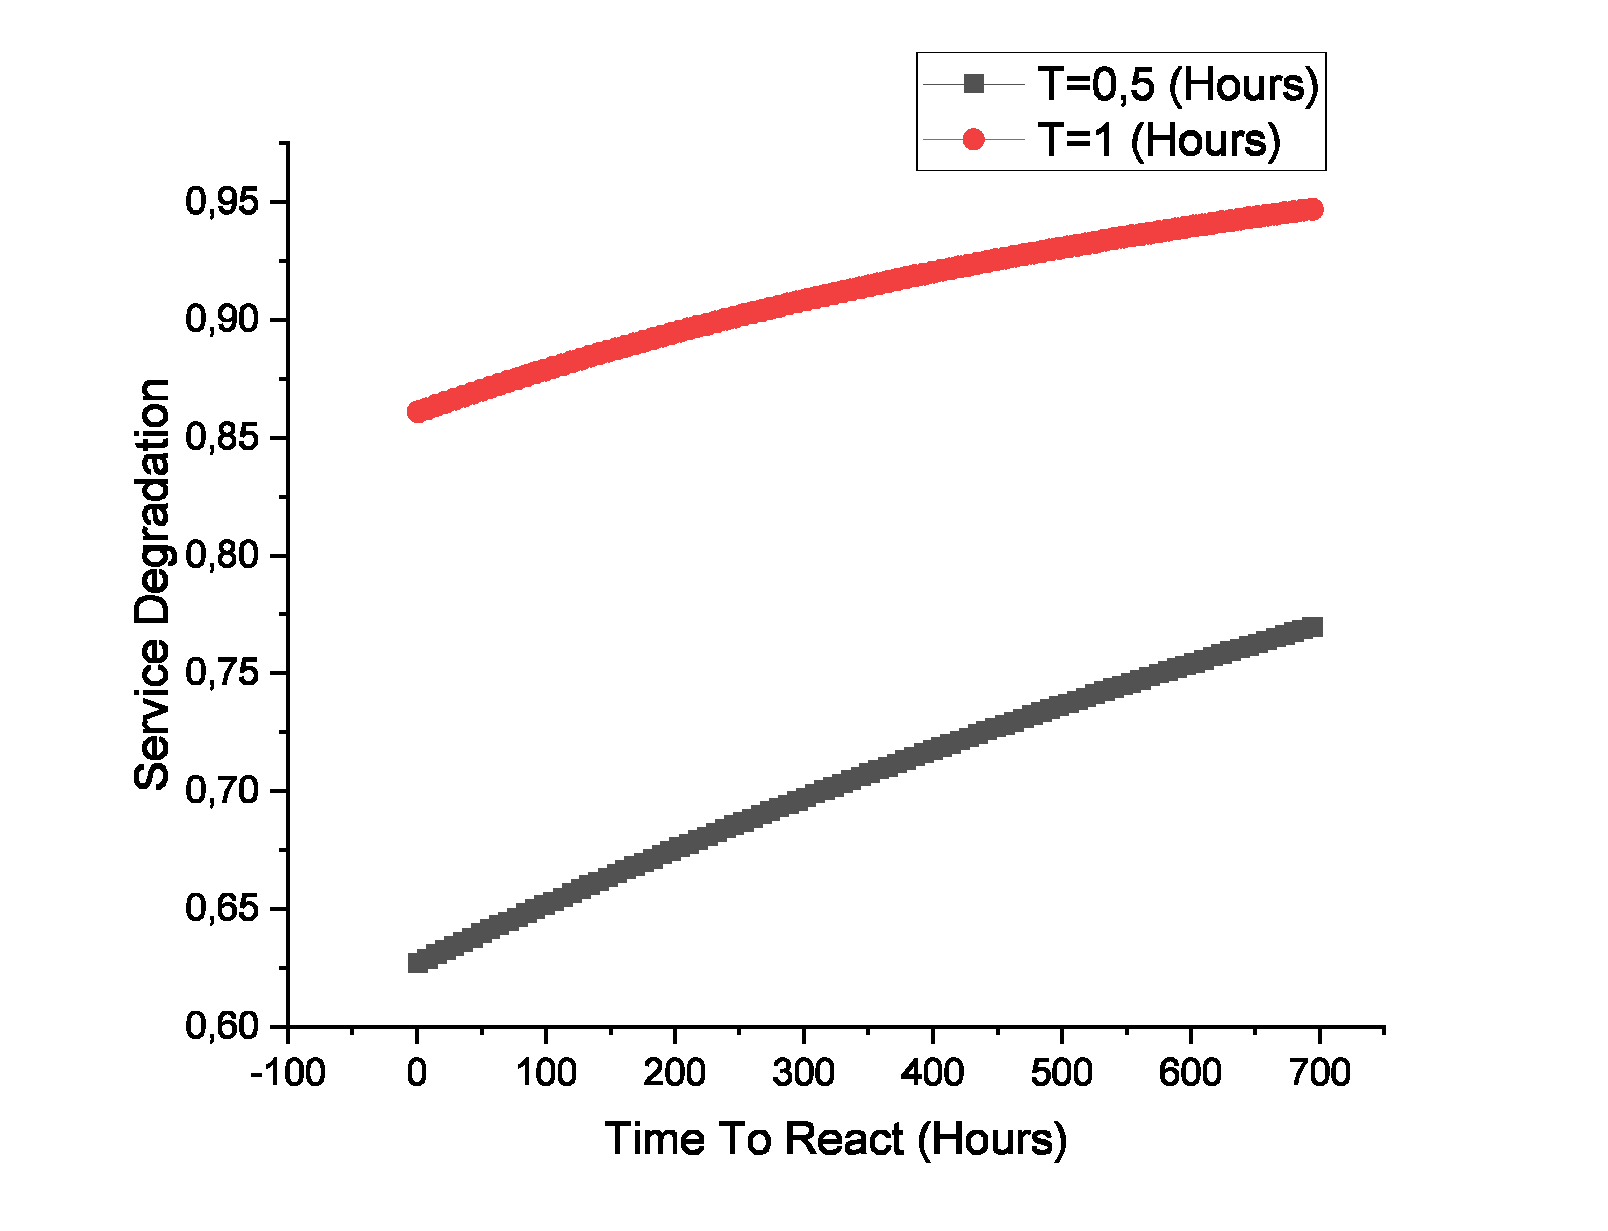
\includegraphics[width=250pt, height =180pt]{Graph1.pdf}
    \caption{Verification of Property \ref{eq1} wit MTTR.}
    \label{fig:02}
   \end{minipage}

               \end{tabularx}
\end{figure}

The results of verifying Property \ref{eq1} are depicted in Figure \fig{fig:01}. The system's ability to rescue the person decreases as time progresses. This is expected, as the SAR/Galileo service may not be able to effectively respond to the distress situation over longer durations. Figure \fig{fig:01} illustrates this system degradation over a period of 0 to 1 hour. It is important to note that our modeling considers degradations that can be detected within a 24-hours.

These results do not demonstrate the possibility that the system does not fully encompass the state of the human in terms of their reaction to danger, such as the Mean  Time To React to danger (MTTR). To address this limitation, we augment the model with a module that represents the human's status in response to a crisis in a one-month calendar. This module incorporates a formula for the rate of urgent response: 

\begin{equation*}
\lambda_{h} = MTTR / Month 
\end{equation*}

So, the model is augmented by human behavior, as shown in \lst{exampleinprism}, and the label \quot{\textcolor{red}{\emathtt{Rescued}}} includes human ability degradation.

\lstdefinestyle{framed}
{
	frame=lrb,
	mathescape,
	numbers=left,
	belowcaptionskip=-1pt,
	xleftmargin=3.11em,
	xrightmargin=0.03cm,
	framexleftmargin=3em,
	framexrightmargin=0pt,
	framextopmargin=5pt,
	framexbottommargin=5pt,
	framesep=0pt,
	rulesep=0pt,
	numbers=left,
}

\lstset{
    breaklines=true,
    style=framed,
    escapeinside={<@}{@>},
    morekeywords={void, int, public, private, class, protected, submodules, network, connections, const, init, int, bool, double, module, rewards, endrewards, endmodule},
    basicstyle=\scriptsize\ttfamily,
    keywordstyle=\bfseries\color{blue},
    morecomment=[f][\color{green!70!black}][0]{/*},
    morecomment=[l][\color{green!30!black}]{//},
    label=queueemodel
}

\begin{figure}[!htb]
\begin{minipage}{9cm}
\begin{lstlisting}[style=framed,
	caption=The Human Status,
 	label=exampleinprism]
module Human_Status
    Human_Status_s : [0..3] init 3;
    [] Human_Status_s>0 -> lambda_h:(Human_Status_s'=Degraded); 
endmodule
\end{lstlisting}
\end{minipage}
\end{figure}

We observe that the system's ability to rescue the person in distress decreases as the MTTR increases (within time windows of T=0.5 and T=0.1 of \fig{fig:01}). While this may seem intuitive, the verification process mathematically confirms this observation. Furthermore, the results demonstrate that the system's effectiveness depends on its capability to rescue the person in danger and crucially relies on the person's timely response to the crisis.

